\documentclass[11 pt]{article}

\usepackage[normalem]{ulem}
\usepackage{algorithm2e}
\usepackage{amsmath}
\usepackage{amssymb}
\usepackage{booktabs}
\usepackage{caption2}
\usepackage{cite}
\usepackage{color}
\usepackage{epsfig}
\usepackage{fancyhdr}
\usepackage{fullpage}
\usepackage{graphics}
\usepackage{graphicx}
\usepackage{hhline}
\usepackage{hyperref}
\usepackage{listings}
\usepackage{moreverb}
\usepackage{multirow}
\usepackage{pgfplots}
\usepackage{psfrag}
% \usepackage{subfigure}
\usepackage{tabu}
\usepackage{verbatim}
\usepackage{wrapfig}
% defines
\newcommand{\etc}{etc.\xspace}
\newcommand{\ie}{i.e.,\xspace}
\newcommand{\eg}{e.g.,\xspace}
\newcommand{\etal}{\emph{et~al.}\xspace}
%\newcommand{\comment}[1]{{\color{gray}[\textsf{#1}]}}
\newenvironment{packed_enum}{
  \begin{itemize}
  \setlength{\topsep}{0pt}
  \setlength{\itemsep}{1pt}
  \setlength{\parskip}{0pt}
  \setlength{\parsep}{0pt}
  \setlength{\parindent}{0pt}
}{\end{itemize}}

\long\def \ignoreme#1{}

% \usepackage[usenames]{color}
\usepackage{color}
\definecolor{gray}{rgb}{0.5,0.5,0.5}
\definecolor{dkgreen}{rgb}{0,0.6,0}
\definecolor{blue}{rgb}{0,0,1}
\definecolor{mauve}{rgb}{0.58,0,0.82}
%\ignoreme{
\newcommand{\alex}[1]{{\color{red}\bf [AO: #1]}}
\newcommand{\milos}[1]{{\color{red}\bf [MP: #1]}}
\newcommand{\alenka}[1]{{\color{red}\bf [AZ: #1]}}
\newcommand{\todo}[1]{{\color{red}\bf \ \\\noindent TODO: #1}}
%}
%\newcommand{\be}{\begin{equation}}
\newcommand{\ee}{\end{equation}}

\def\denseitems{
  \itemsep1pt plus1pt minus1pt
  \parsep0pt plus0pt
  \parskip0pt
  \topsep0pt
}
\leftmargini 1em
%  \leftmarginii-1em
%  \leftmarginiii-1em
%  \leftmarginvi-1em

\newcommand \co {\tt \small}

\setlength{\textheight}{9in}
\setlength{\textwidth}{6.5in}
\setlength{\topmargin}{0pt}
\setlength{\evensidemargin}{1pt}
\setlength{\oddsidemargin}{1pt}
\setlength{\headsep}{10pt}
\setlength{\parskip}{0ex}
\voffset -0.2in

\clubpenalty=10000
\widowpenalty=10000

\newcommand{\beq}{\begin{equation}}
\newcommand{\eeq}{\end{equation}}
\newcommand{\bsp}{\begin{split}}
\newcommand{\esp}{\end{split}}
\newcommand{\bal}{\begin{align*}}
\newcommand{\eal}{\end{align*}}
\newcommand{\bml}{\begin{multline}}
\newcommand{\eml}{\end{multline}}
\newcommand{\bi}{\begin{enumerate}}
\newcommand{\ei}{\end{enumerate}}
\newcommand{\bea}{\begin{eqnarray}}
\newcommand{\eea}{\end{eqnarray}}
\newcommand{\bc}{\begin{center}}
\newcommand{\ec}{\end{center}}
\newcommand{\denotes}{\stackrel{\triangle}{=}}
\newcommand{\la}{\langle}
\newcommand{\ra}{\rangle}
\newcommand{\nn}{\nonumber}
\newcommand{\bPsi}{{\mbox {\boldmath $\Psi$}}}
\newcommand{\her}{{\scriptscriptstyle H}}

\DeclareGraphicsExtensions{.png}

\newlength\figureheight
\newlength\figurewidth
% Density adjustment parameters

% Controls the amount of additional space between paragraphs
\parskip 0.4\baselineskip
% Controls the spacing between lines (1.00 is normal spacing)
\linespread{1.00}

%%% PAGE SETUP
\special{papersize=8.5in,11in}
%\special{portrait}

% FORMATTING
%==============================================================
% Note that this is not perfectly 1 inch margin (larger) but
% ps2pdf shrinks it a bit so the end result has perfect 1-inch margins
%\setlength{\oddsidemargin}{-0.1in}
%\setlength{\evensidemargin}{-0.1in}
%\setlength{\textwidth}{6.8in}
%\setlength{\textheight}{9.2in}
%\setlength{\topmargin}{-0.2in}
%\setlength{\headheight}{0in}
%\setlength{\headsep}{0in}
%\addtolength{\footskip}{-5pt}

\setlength{\oddsidemargin}{0in}
\setlength{\evensidemargin}{0in}
\setlength{\textwidth}{6.5in}
\setlength{\textheight}{9.0in}
\setlength{\topmargin}{0in}
\setlength{\headheight}{0in}
\setlength{\headsep}{0in}
%\addtolength{\footskip}{-5pt}

\marginparsep 0in
\marginparwidth 0in
\footskip 0.5in
\columnsep 0.22in
\parindent 0in
\textfloatsep 0.10 in
\dbltextfloatsep 0.10 in
\floatsep 0.10 in
\dblfloatsep 0.10 in
\intextsep 0.10 in
\sloppy

%\renewcommand{\baselinestretch}{0.95}
\newcommand{\SF}[1]{{\fontsize{6}{6pt}\sffamily#1}}

% Changes to Times Roman font, which is one of the fonts allowed by NSF
\usepackage{mathptmx}

% For research.gov proposals pages should not be numbered,
% their system adds page numbers as it puts together the overall proposal document
\usepackage{nopageno}

\renewcommand{\footnote}[1]{\errmessage{Footnotes are not allowed in an NSF Project Description!}}

%==============================================================



%%===========================================================================
\makeatletter
\renewcommand{\@seccntformat}[1]{
\hspace{-2pt}{\csname the#1\endcsname}.\hspace{0.5em}}
\makeatother

\makeatletter
\renewcommand{\section}{\@startsection
  {section}               % name
  {1}                     % level
  {0pt}                   % indent
  {0.4\baselineskip}      % beforeskip
  {0.1\baselineskip}         % afterskip
  {\fontsize{12}{\baselineskip} \rmfamily \bfseries}} % style
\makeatother

\makeatletter
\renewcommand{\subsection}{\@startsection
  {subsection}            % name
  {2}                     % level
  {0pt}                   % indent
  {0.3\baselineskip}      % beforeskip
  {0.1\baselineskip}         % afterskip
  {\fontsize{12}{\baselineskip} \rmfamily \bfseries}} % style
\makeatother

\makeatletter
\renewcommand{\subsubsection}{\@startsection
  {subsubsection}               % name
  {3}                     % level
  {0pt}                   % indent
  {0.2\baselineskip}         % beforeskip
  {0.1\baselineskip}                   % afterskip
  {\fontsize{11}{\baselineskip} \rmfamily \bfseries}} % style
\makeatother

%%===========================================================================

\font\tenhv  = phvb at 8pt

\renewcommand{\floatpagefraction}{0.7}
\renewcommand{\dblfloatpagefraction}{0.7}

\renewcommand\refname{References Cited}


%\renewcommand{\captionfont}{\small}
%\setcaptionmargin{0.05\textwidth}
%\setlength{\abovecaptionskip}{10pt}
%\newcommand{\ignore}[1]{}

\begin{document}

% \title{\vspace{-0.5cm}SHF:Medium: Spectral Profiling – Understanding Software Performance without Code Instrumentation}
% \author{Project Description}
%  \date{}
%  \maketitle
%  \vspace{-0.6cm}

\begin{center}
{\Large \textbf{SHF:Medium:Making Analog Side Channels a First-Class Consideration in Architecture-Level Design}}
\end{center}

\section{Introduction}
Analog side-channels (power, electromagnetic, acoustic, etc.) have long been a potential source of attacks that circumvent traditional protections and security measures~\cite{217605,Backes:2010:ASA:1929820.1929847,Balasch2015DPABA,10.1007/978-3-319-66787-4_27,4812164,Chari:2002:TA:648255.752740,Genkin:2016:EKE:2976749.2978353}. This is especially a problem for cyber-physical systems (CPS) and Internet-of-Things (IoT) systems which often contain sensitive data, such as sensor data, login information for over-the-network management of the system and/or accessing back-end cloud infrastructure, and are often placed in publicly accessible  locations. For some side-channels, such as electromagnetic (EM) emanations, physical proximity can be leveraged to attack systems that are considered to be physically secure but are located near publicly accessible locations, e.g., in-wall ``smart building'' sensors, security cameras, etc~\cite{10.1007/978-3-662-48324-4_11,6766222,Camurati:2018:SCE:3243734.3243802,8574570}.
Many such attacks have been demonstrated over the past several decades, followed by countermeasures that prevent specific attacks by modifying the software that has been demonstrated to leak sensitive information. However, the PIs recent analog side channel attacks have shown that both attacks and mitigation are becoming increasingly dependent on microarchitectural behavior and potentially fragile to future microarchitectural changes~\cite{217605,Monjur21}.
Unfortunately, early-design tools such as cycle-accurate simulators~\cite{Li:2009:MIP:1669112.1669172,Li:2011:CAM:2132325.2132479,509850,Ardestani:2013:EFM:2495252.2495480,Binkert:2011:GS:2024716.2024718,sesc,5982026,carlson2014aeohmcm}  do not model analog side channel signals, so these side channels can only be considered when they can be physically measured on already-fabricated chips. At that time, however, time-to-market concerns prevent introduction of overall design changes that would adjust the design tradeoffs in a more desirable direction. Additionally, most software developers have neither the know-how nor the equipment to assess their software’s potential vulnerability to analog side channels, so such considerations are typically either absent or qualitative/abstract when software is designed, giving first-mover advantage to attackers, and resulting in mitigation via localized patches, which themselves are becoming increasingly microarchitecture-dependent.

Ideally, the potential for information leakage through analog side channels and ``breaking'' existing software mitigation approaches would be considered in early stages of design for both hardware and software, guided by tools that can predict the impact a specific design has on analog side channels. This would be analogous to how performance and power consumption are predicted by cycle-accurate simulators, which allows the tradeoff between performance, power, and cost to be investigated at design time, years before the first prototype of that processor is fabricated ~\cite{Li:2009:MIP:1669112.1669172,Li:2011:CAM:2132325.2132479,509850,Ardestani:2013:EFM:2495252.2495480,Binkert:2011:GS:2024716.2024718,sesc,5982026,carlson2014aeohmcm} If such efficient-yet-highly-accurate simulation would exist for analog side channels, hardware designers and architects could include analog side-channel leakage among their design considerations~\cite{8416860,Althoff:2018:HII:3276539.3276601,Andrysco:2018:TVC:3243734.3243766,cryptoeprint:2018:808,Rane:2016:SPF:3241094.3241101,nayak2017hop}, compilers could use simulation models to optimize for reduced leakage~\cite{Liu:2015:GHS:2694344.2694385,Rane:2015:RCD:2831143.2831171,Gorman:2017:AON:3123939.3123973}, software designers could detect and mitigate information leakage problems for security-sensitive applications~\cite{Wichelmann:2018:MFF:3274694.3274741,Chen:2017:PDS:3133956.3134058,Wu:2018:ETS:3213846.3213851}, etc.

While there are some tools and metrics to quantify analog side-channel leakages~\cite{Demme:2013:FOM:2485922.2485970,Callan:2014:PMM:2742155.2742179,McCann:2017:TPT:3241189.3241207,Barenghi:2018:SSS:3195970.3196112, yilmaz17tifs}, they are limited due to following reasons: \textit{First}, they are mainly focused on developing metrics to estimate the information leakage itself, i.e., mutual information between the signal and the program secrets, rather than modeling the actual analog signal. Relying only on these metrics rather than analyzing the actual signal, may not be sufficient since these metrics inherently make assumptions about the aspects of the signal the attacker may exploit, i.e., they may not reveal \emph{all} of the information the signal may contain. \textit{Secondly}, existing methods only model the system at \textit{architecture-level}, i.e., associating a (leakage) value to individual instructions based on the ISA, and ignore the micro-architecture activities such as pipeline stages, stall cycles, etc. on the signal. As we have demonstrated in our seminal paper on analog side channel modeling \cite{Nader2020}, this can lead to significant inaccuracy, mainly because the model, by staying at the ISA-level, neglects to account for how that instruction interacts with other instructions and the underlying hardware.  \textit{Thirdly}, by neglecting the impact of micro-architecture, these methods implicitly assume that the entire hardware design is a \textit{single source}, and then only model the analog emanations based on this single source. Such an assumption can lead to large inaccuracies since different micro-architecture components (e.g., cache, register-file, etc.) generate different electromagnetic waves with different polarization and/or phase, and hence, they may have \emph{constructive or destructive} impacts on each other and the overall received signal.

The PIs first attempt to address these challenges and develop microarchitecture-level analog side-channel model was presented in \cite{Nader2020}. The model was a proof of concept that very precise estimation of leakage not only for individual instructions but also for sequences of instructions (when the goal is to assess and improve leakage from a particular piece of code on a set of hardware platforms) is feasible. This model is also the first to asses leakage from a particular part of the system (when the goal is to make the design less ``leaky'') while maintaining the performance advantages of a cycle-accurate simulation relative to a physics-based model. While the proposed model is good enough for demonstrating possibility of modeling analog side channels, this model has many limitations: 1) it does not scale well across different architectures and processor clock frequencies, 2) Needs prohibitively large number of training sequences to cover all possibilities among opcodes and registers, 3) has large number of parameters that need to be estimated from measurements.
\subsection{Proposed Research Work}
To address these issues and consider jointly tradeoff between performance, power, and analog side channels we propose to develop:
\begin{itemize}
\item techniques that allow architecture-level simulators to efficiently generate estimated side channel signals, to help computer architects, researchers, and software developers assess the impacts of microarchitectural and software changes on the tradeoff between performance, power, and side channel leakage.
\item methods for efficient circuit-level exploration of caches and functional units that can be integrated into architecture-level simulators, analogous to how Cacti and McPat are used to obtain per-event latency and power estimates in cycle-accurate simulators.
\item \textbf{Machine learning methods for analog side channel modeling}. In this task we propose to develop machine learning techniques that will allow for analog side channel modeling that is not dependant on collecting measurements on particular processor and are scalable across different processor and memory speeds. Furthermore, we propose to create neural network structure that does not require to observe all possible combinations of instructions in order to model larger sequences of instructions. Finally, we propose to develop methods for ``calibration'' of simulation parameters against measured signals from real systems.
 \end{itemize}
 %If successful, our work will demonstrate the feasibility of modeling analog side-channels at the microarchitectural level and provide proof-of-concept integration of such modeling into a cycle-accurate simulator. This will allow analog side channels to become a first-class consideration, along with performance and power, in processor designs, allowing computer architects to avoid introducing significant new vulnerabilities and ``breaking'' existing software mitigation, and possibly even to reduce leakage and/or enable new mitigation. It would also allow programmers and even compilers to include analog side channel considerations in their tradeoff space during design and/or optimization.
\subsection{Broader Impact}
We expect that our results will help the inclusion of analog side channels among early design considerations and will help reduce the cost of side-channel resistant designs by addressing side-channel-related problems early in the design process, when side-channel resilience may be improved (or preserved) with little or no sacrifice in performance, power, cost, weight, etc. The proposed work is inherently interdisciplinary, combining expertise in computer architecture and circuits, hardware security, electromagnetic, and signal processing. Thus this research has the potential to improve the state of the art and have broader impacts in all these areas. Also, participating students will be working in a truly multidisciplinary context, which will broaden their expertise in ways otherwise not possible as well as {\bf broaden participation in computing}. The proposal also includes 1) developing an interactive demonstrator for the general public, to educate and raise awareness about several key cyber-security concepts and issues, 2) visits and activities in local schools to improve K-12 education and participation of women and minorities in STEM, and 3) course and curriculum development activities at the undergraduate and graduate level.
\section{Related Work}
There is a large body of work focused on preventing particular side-channel attacks, e.g., ~\cite{Backes:2010:ASA:1929820.1929847,Nazari:2017:EED:3079856.3080223,Demme:2013:FOM:2485922.2485970,Han:2017:WMB:3133956.3134081,Liu:2016:CET:2976749.2978299,6987331,He:2017:SYC:3123939.3124546,217605,Monjur21}, either by removing the tie between sensitive information and the side-channel signal, or by
trying to make the signal more difficult to measure. However, such work mostly focuses on preventing a particular side
channel attack in a very specific piece of code and are less focused about the fundamental relationship between the hardware, software, and the side-channel signal.

Strategies for quantifying potential side channel exposure at the micro-architectural and architectural levels are still
an open problem. Existing work proposed different methods and/or metrics to estimate the leakage either for a specific type of side-channel (e.g., cache, power, EM, etc.) or alternatively, as a generic framework to estimate the overall leakage for any given side-channel.

Side-Channel Vulnerability Factor (SVF)~\cite{Demme:2013:FOM:2485922.2485970} measures how the side-channel signal correlates with
high-level execution patterns (e.g., program phase transitions).
While this metric allows overall assessment of the
``leakiness'' of a particular system and application over a
given side-channel, it provides limited insight to 1) computer
architects about which architectural and microarchitectural
features are the strongest leakers, and to 2) software developers
about how to reduce the side-channel leakiness of their
code.

To address these limitations, Signal Available to Attacker (SAVAT) method~\cite{Callan:2014:PMM:2742155.2742179} was proposed. SAVAT measures the side-channel signal (particularly EM and power from laptops) created by a specific single-instruction difference
in program execution, i.e., the amount of signal made available
to a potential attacker who wishes to decide whether the
program has executed instruction/event A or instruction/event B. These measurements can be used
to determine the potential for information leakage when
execution of individual instructions or even sections of code
depend on sensitive information. Unfortunately, SAVAT only models the system at ISA-level and ignores the underlying relation of each instruction to the hardware or other instructions in the sequence. Extensions of SAVAT that include modeling instructions overlapping in pipeline have been proposed in \cite{baki17}, \cite{Baki_2020a}.

Similar to SAVAT, McCann \textit{et al.}~\cite{McCann:2017:TPT:3241189.3241207} proposed a modeling technique capable of
producing a leakage metric at instruction-level for power (and/or
EM) side-channel signals on ARM M0/M4 cores. To estimate the leakage for individual instructions, the proposed method  only requires knowledge about different characteristics of the system at ISA-level such as data-dependent effects of neighboring
instructions in a sequence, register effects, bit-flips, etc. Similar to SAVAT, while the method proposed by McCann \textit{et al.}~\cite{McCann:2017:TPT:3241189.3241207} provides interesting insights about possible sources of leakage, it also ignores the effects of micro-architecture events such as cache miss, branch miss-prediction, etc. on the signal.

The method proposed by Barenghi and Pelosi~\cite{Barenghi:2018:SSS:3195970.3196112} calculates the leakage for individual instructions by measuring the power consumption between two consecutive cycles and employs the Pearson correlation coefficient between the two measurements. To calculate the leakage, in addition to leveraging the ISA-level information, pipeline model was also used. However, the framework did not consider any micro-architecture events, nor pipeline stalls and only accounts the number of cycles that takes for each instruction to execute. It also did not model the individual effect of each stage on the others and the overall signal.

Another approach to quantifying side channel leakage is to use information theory and estimate capacity of analog side channels. Millen was the first to establish a connection between Shannon's information theory and information flow models in computer systems~\cite{Millen87}
and calculated the capacity (maximum possible data rate) of such a side-channel.
However, that model assumes a synchronous channel (where information is transmitted at a constant rate that is known to the receiver),
and this is not a realistic assumption for analog side-channels in computer systems, where the timing of execution in the spy program varies
due to a number of hardware features (e.g., pipeline stalls, dynamic scheduling of instructions, cache hits and misses, branch prediction, etc.).
Additionally, analog side-channels often include insertion, deletion, and errors, e.g., interrupts and other system activities often insert activity into the timeline of the spy program's execution. There are many papers that discuss bounds on the capacity of channels corrupted by synchronization errors
~\cite{Wang05}, \cite{Anderson98}, \cite{Crespi13}, \cite{Davey01}, \cite{Ramachandran11}, \cite{Kirsch10}, \cite{Hu10}, bounds on the capacity of channels corrupted with synchronization and substitution errors \cite{Verdu10}, \cite{Duman13}, \cite{Tarokh12}, or bounds on the capacity when codewords have variable length but no errors in the channel \cite{Verdu10}, \cite{Shannon:InfoPaper}, none of them provides the answer to how much information is ``transmitted'' by execution of particular sequence of instructions that do not have equal timing and are transmitted through erroneous channel.
The first attempts to answer this question were presented in \cite{baki18icassp,baki18milcom}, where covert channels are generated, and upper and lower leakage capacities were derived. In \cite{baki17}, a side channel leakage capacity is derived for a discrete memoryless channel where it was assumed that each transmitted quantum of information (i.e., instruction in the code) is mutually independent but do not have equal length. Although all these papers make an important step toward assessing information leakage from side-channels, they fall short of considering the relationship among sequence of instructions, which is a result of program functionality as well as a processor pipeline depth, which impacts how much signal energy will be emanated.
In \cite{Baki_2020a}, side-channel information capacity created by execution of series of instructions (e.g., a function, a procedure, or a program) in a processor is derived. To model dependence among program instructions in a code, we use Markov Source model, which includes the dependencies that exist in instruction sequence since each program code is written systematically to perform a specific task. The presented  framework  considers processors as the transmitters of a communication system with multiple antennas. The antennas correspond to different pipeline stages of any processor. Moreover, inputs of the transmitter show dependency based on a Markov model which reflects the practicality of a program. Using this setup, we have obtained the channel capacity of a communication system which represents the severity of the side channels. However, none of these approaches provide enough details to model analog side channels taking into consideration microarchitecture details.

Another body of work related to this proposal are the cycle-accurate models/tools to simulate power and/or microarchitecture~\cite{Li:2009:MIP:1669112.1669172,Li:2011:CAM:2132325.2132479,509850,Ardestani:2013:EFM:2495252.2495480,Binkert:2011:GS:2024716.2024718,sesc,5982026,carlson2014aeohmcm}. While these models can accurately model the power consumption at each cycle, they are different from this work and hence may not be a proper tool for simulating analog side-channel signals for two main reasons: \textit{First}, while these methods do consider the activity factor to calculate power, they often treat all the bit-flips equally. However, as shown in \cite{Nader2020}, depending on the design, not all flips equally contribute to the overall signal. Ignoring this fact can lead to inaccurate modeling. \textit{Second}, depending on the architecture, different stages might have different effect on each other and the overall signal. Without properly modeling these effects, the overall signal can not be modeled.

Also related to this work are work on leveraging EM signals for program profiling, tracking, and analysis~\cite{7783762,Gorman:2017:AON:3123939.3123973,Elvan2021,Zop, Zop2,Moumita2018,Moumita2022}. Spectral Profiling methods~\cite{7783762,Zop,Zop2,Elvan2021} tracks program execution at different granularity from loops \cite{7783762}, to basic blocks \cite{Zop,Zop2} and individual instructions \cite{Elvan2021}. \textsc{EMProf} profiles memory \cite{Moumita2018} and \textsc{Primer} profiles interrupts \cite{Moumita2022}, both leveraging electromagnetic (EM) emanations from devices. By continuously analyzing these EM emanations, \textsc{EMProf} identifies where in the signal's timeline each period of stalling begins and ends, allowing it to both identify the memory events that affect performance the most (LLC misses) and measure the actual performance impact of each such event (or overlapping group of events). Because \textsc{EMProf} is completely external to the profiled system, it does not change the behavior of the profiled system in any way, and requires no hardware support, no memory or other resources, and no instrumentation on the profiled system. Similarly, \textsc{Primer} analyzes the device's external EM side-channel signal in real-time, without any interference with the device's program execution, while providing a detailed analysis of not only the overall overhead created by interrupts, but also their distribution over time (i.e., exact occurrence of interrupts in program execution time-line). As the CPU follows a generic procedure to handle such asynchronous system events, our approach can be generalized and applied to all non-deterministic interrupts across multiple platforms. More details on both methods are presented in following sections. All these methods are complimentary to this proposal and combined with proposed modeling tool can enhance leakage estimation, compiler development, etc.

However, none of them address the need for developing microarchitecture-level analog side-channel tool such that allows for integration of such modeling into a cycle-accurate simulator. This, in turn, would allow analog side channels to become a first-class consideration, along with performance and power, in processor designs, allowing computer architects to avoid introducing significant new vulnerabilities and ``breaking'' existing software mitigation, and possibly even to reduce leakage and/or enable new mitigation.

\section{Preliminary Results}
\label{sec:preliminary_results}
The PIs are the first to attempt to address these challenges and develop microarchitecture-level EM side-channel model \cite{Nader2020}.

Fundamentally, EM side-channel signals are created due to \textit{bit-flips} at the transistor-level~\cite{VANECK1985269,6766222}.
In principle, all transistors and metal-layer interconnect components contribute to the signal, thus the signal could be modeled using all transistors and on-chip wires as predictor variables, which {\em should} be highly accurate but is practically infeasible.
As a result, the main challenge in model-building is to select (or discard) potential predictors in a systematic manner, to achieve a trade-off where feasibility (or even efficiency) is achieved without a major sacrifice in accuracy.

To accurately simulate EM signals, we model micro-architectural components as \textbf{\textit{independent}} sources of EM emanations and then further group these units in each pipeline stage as an individual source. We use pipeline stages as the sources mainly because we observed that each instruction has different footprint in each cycle, and the side-channel generated at each cycle is a combination of these activities in \textit{ALL} stages. Using this methodology, we model a multi-input (pipeline stages), single-output (EM signal) system (MISO).

Leveraging this approach, the \textbf{challenges} are \textbf{\textit{a)}} \textit{how to model the signal for individual sources}, and \textbf{\textit{b)}}\textit{how to properly combine the signals} generated by each source to accurately form the side-channel signal.

\subsection{Signal Amplitude for Individual Sources}
In practice, there are two contributors in creating EM side-channel signals for each pipeline stage. The first group of contributors, which we call \textit{instruction-dependent} activities, are caused by the switching activities of micro-architectural units (e.g., register-file, ALU, etc.) that are utilized in that stage (e.g., whether the register-file is being written or not).

The second group, \textit{data-dependent} activities, are created due to bit-flips on the data-bus, address-bus, and any other registers that hold operand's values. These bit-flips are independent from the instruction-type but are dependent to the previous state of the bus. In the following, we will describe how we \textit{independently} measure each of these two groups. \\

\noindent \textbf{Instruction-Dependent Activities}. To independently measure these groups, we first minimize the effect of the \textit{data-dependent} activities by setting all the operands, addresses, and immediate values to zero. This approach enables us to measure the \textit{baseline} signal for each stage which is \textit{only} created by the switching activities of the micro-architectural units used in that stage.
\begin{wrapfigure}{l}{0.4\textwidth}
	\centering
	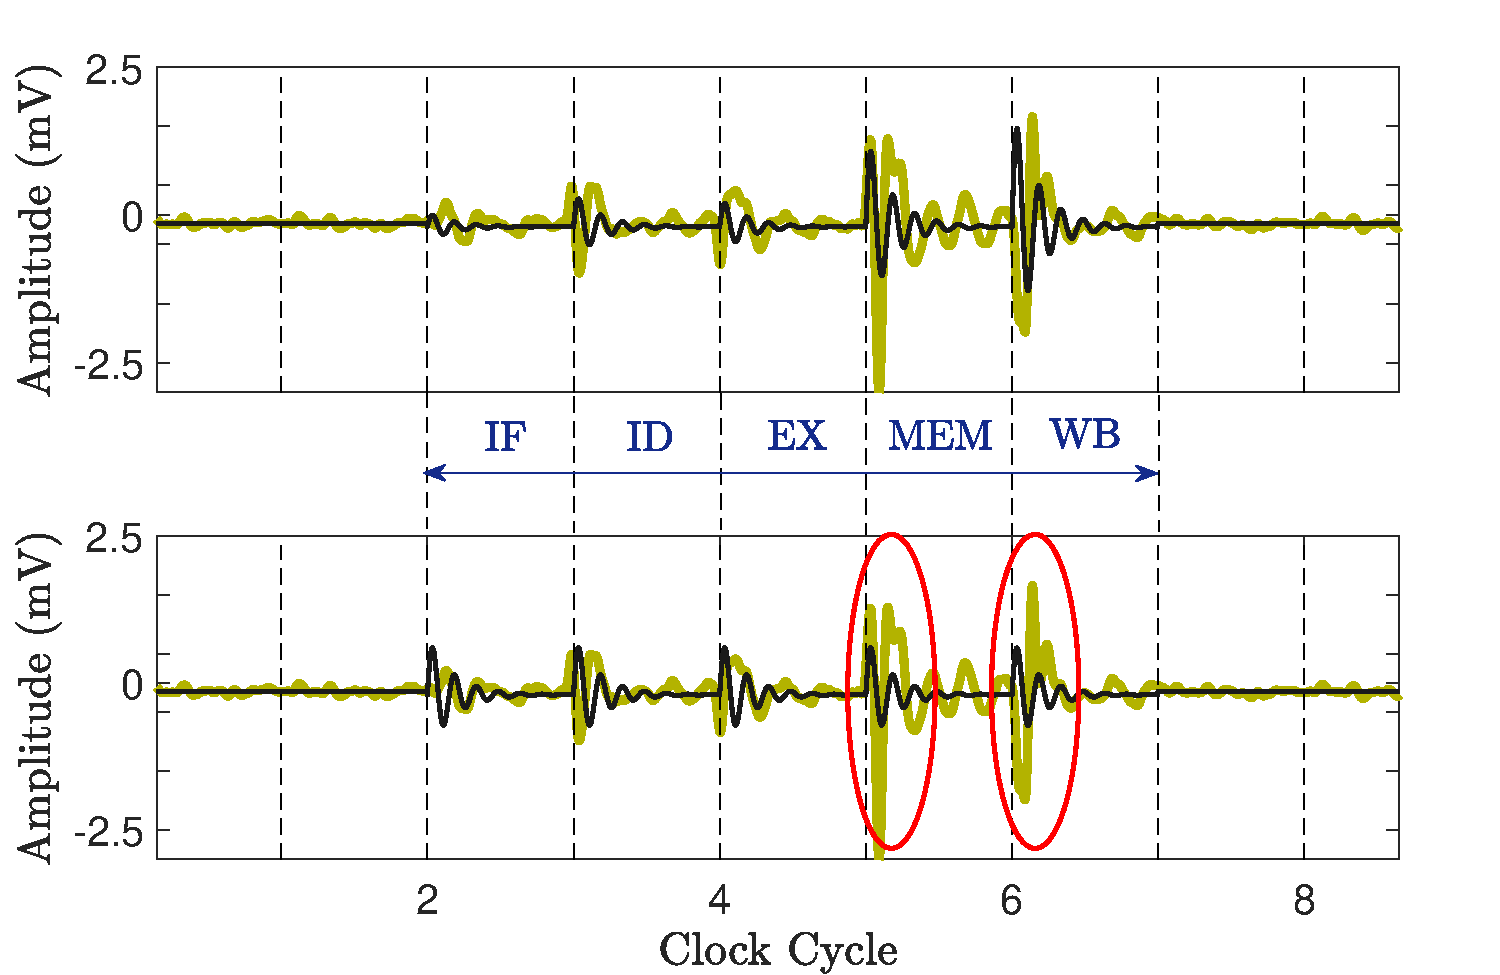
\includegraphics[width=0.4\columnwidth,clip]{figure/amp2.pdf}
	\caption{The signal amplitude for an {\tt ADD} as it progress in the pipeline (while all other instructions are {\tt NOP}). The actual signal is shown in light color (green). Darker color (black) shows the simulated signal when considering each pipeline stage as a separate source (top), and when considering the entire processor as a single source (bottom), and the largest differences between the two are pointed out using red ellipses.}
	\label{fig:amp}
	\vspace{-5mm}
\end{wrapfigure}

After decoupling the data-related activities from the signal, the second challenge is to minimize the effects of other stages on the generated EM signal. Recall that we mentioned \textit{ALL} pipeline stages contribute to the overall signal, however, ideally we want to be able to measure the effect of each stage \textit{separately} so that we can use them as the basic-blocks to reconstruct the overall signal. To achieve that, we use {\tt NOP}
instruction as the \textit{baseline} since it has the minimum possible switching activity, and then create {\tt NOP} $\rightarrow$ {\tt inst} $\rightarrow$ {\tt NOP} instruction sequence (for all instructions), while operands for {\tt inst} are all set to $r1$ (and $r1 = 0$). Using this method, no data/operand-dependent bit-flips are created, but register-file, ALU, etc. may be used (depending on the instruction type). We then measure the signal amplitude for all instructions and every pipeline stages. We call this \textbf{\textit{baseline hardware amplitude}} or \textbf{\textit{$A$}}.

Figure~\ref{fig:amp} shows how the (actual) EM signal (shown in green/light color) changes as an {\tt ADD} instruction progresses through the pipeline while all the other instructions are {\tt NOP}. Using Equ.~\ref{equ:em} \cite{Nader2020} and {\tt NOP}$\rightarrow$ {\tt inst}$\rightarrow$ {\tt NOP} instruction sequence, we used our simulator to generate the signal. 
\begin{equation}
y(t) = \sum_{n=0}^{+\infty} x[n] \sin(\frac{2\pi(t-nT)}{T_0})  e^{-\theta(t-nT)}  \mathtt{u}(t-nT).
\label{equ:em}
\end{equation}
This equation represents two main effects we observed in the analog side-channel signal: 1)
\textit{switching activity in a processor is synchronized to its clock} and most of the switching happens right after the positive/negative edge of the clock, which implies that activity is not evenly spread over a cycle and a decaying function can be used to model clock activities; 2) \textit{the received signal is also exposed to oscillations with decreasing magnitude}, i.e., small signal variations can be modeled as sinusoidal oscillations.
Further, to show why individual stages should be modeled separately, Figure~\ref{fig:amp} (bottom) shows the simulated signal when the ``average'' amplitude is used for all stages. As can be seen, failing to model each stage individually (as used in previous work~\cite{McCann:2017:TPT:3241189.3241207}) can lead to significant inaccuracies in some stages (note that using \textit{max} instead of \textit{average} also leads to similar inaccuracies).  \\

\noindent \textbf{Data-Dependent Activities}. Once the baseline amplitude is measured, the next step is to find how this amplitude changes as the number of bit-flips changes due to value/operand used in the instruction and the previous state of the bus/register. Intuitively, the more bit-flips, the higher the amplitude should be thus we define \textit{activity-factor}, $\alpha$, as a \textbf{\textit{scaling factor}} to the baseline activity, $A$.
To find $\alpha$, we first treat each bit-flip \textit{equally}, and assume that each bit-flip has similar effect on the signal amplitude. We then calculate $\alpha$ as:
\begin{equation}
\alpha = 1 + \frac{(\mathit{flips}_{new} - \mathit{flips}_{base})}{\mathit{flips}_{total}},
\end{equation}
where $\mathit{flips}_{new}$ is the total number of flips for the current instruction,  $\mathit{flips}_{base}$ is the total number of flips when previous instruction is {\tt NOP}, and $\mathit{flips}_{total}$ is the maximum possible number of flips for the current instruction. Using this equation, we then define $A' = \alpha\times A$, and use it to simulate the signal. Figure~\ref{fig:alpha} (bottom) shows the original signal (shown in light green), and the simulated signal using this approach (shown in black) for the similar {\tt NOP}$\rightarrow$ {\tt inst}$\rightarrow$ {\tt NOP} instruction sequence discussed in the previous section. As can be seen in the figure (bottom), this \textit{``averaging''} modeling can not accurately predict the amplitude of the signal which indicates that \emph{not all the bit-flips have the similar impact on the amplitude}. Our further investigation confirmed this theory. Particularly, we found that flips in the output of the ALU and memory have the most significant impacts on the signal. We believe this difference is mainly due to the different physical parameters of transistors and/or lengths of the connecting wires.
\begin{wrapfigure}{l}{0.4\textwidth}
	\centering
	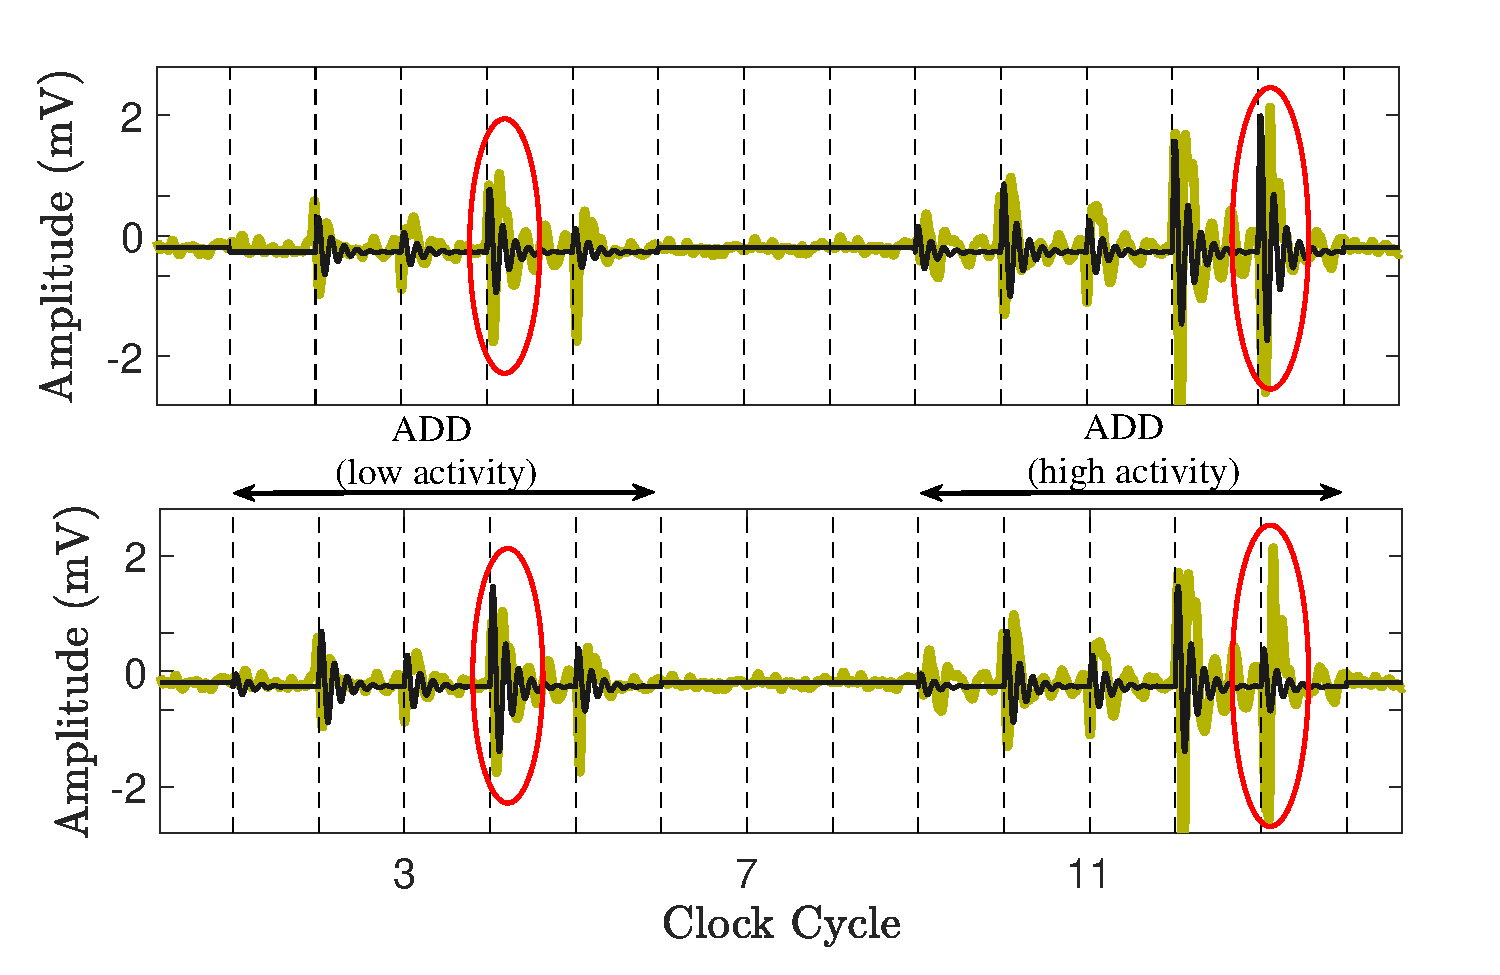
\includegraphics[width=0.4\columnwidth]{figure/alpha2.pdf}
	\caption{Effect of the \textit{activity factor} on the amplitude. The actual signal shown in green. The simulation is shown in black when activity factor is modeled using a linear regression model (top) and when an \textit{average} activity is used (bottom).}
	\label{fig:alpha}
\end{wrapfigure}

Using this observation, to systematically calculate the activity factors, we use a \textit{linear regression} model:
\begin{equation}
\alpha = \delta + \mathcal{T}\times c + \epsilon,
\end{equation}
where $\mathcal{T}$ is a vector of transition bits across all the existing registers in the targeted pipeline stage, $\delta$ and $\epsilon$ are the vector of scalar intercept and error terms respectively, and $c$ is the vector of activity factors to be predicted by the model. As mentioned before, $\alpha$ is the scaling factor for the baseline amplitude, $A$, thus $\alpha = A_{meas}/A_{simul}$.  Note that to find $\mathcal{T}$, a detailed micro-architecture model is needed to track all the bit-flips for every gate in the processor (except cache/memory). However, to significantly reduce the complexity and simulation time, the size of $\mathcal{T}$ can be reduced using the step-wise regression method~\cite{f-test} where, iteratively, the size of the fitted model (i.e., $\alpha$ and $\mathcal{T}$ in our case) is reduced using standard statistical metrics such as F-tests~\cite{f-test}. In other words, since \emph{not all the bit-flips have statistically significant impact on the emanated signal}, the non-contributing factors can/should be removed from the model.  In our processor, using this method we managed to reduce the size of $\mathcal{T}$ by more than 65\%.

Figure~\ref{fig:alpha} (top) shows the simulated signals when the linear regression (LR) model is used for activity factors. Compared to the averaging method (bottom), using LR has significantly improved the simulation accuracy.

\subsection{Multi-Input Modeling}
Once the signal amplitude for individual sources are calculated, the next step is to combine the signals generated by these individual sources to create the simulated EM signal.
In principle, the generated EM signal is the \textit{superposition} of individual waves thus depending on each source's phase, the superposition of each pair can be either \textit{constructive} or \textit{destructive}. Using this fact, the overall signal can be approximated as a \textit{linear} combination of these individual sources where the coefficients may vary between $\pm$1, depending on the phases.

\begin{wrapfigure}{l}{0.4\textwidth}
	\centering	
	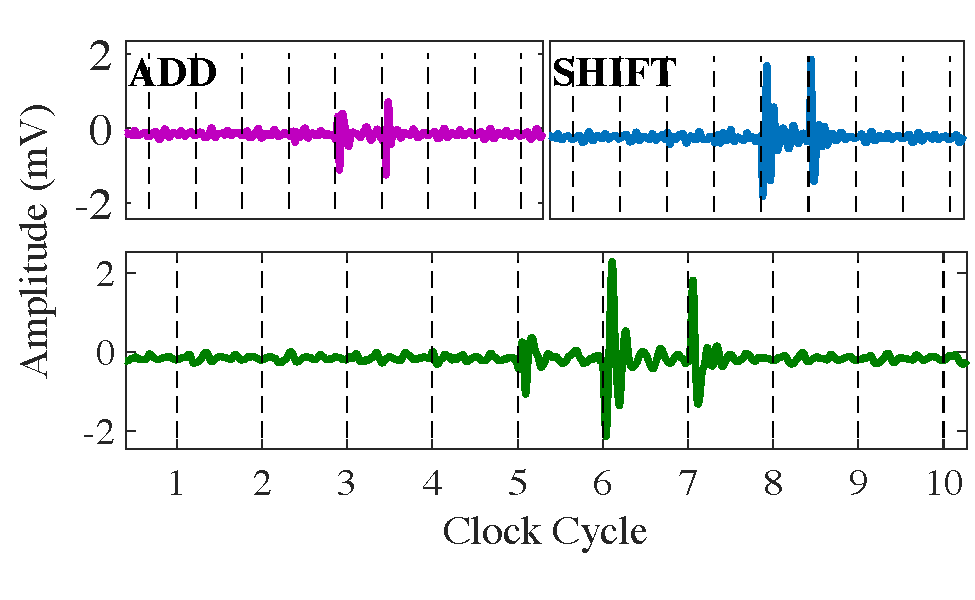
\includegraphics[width=0.4\columnwidth]{figure/miso.pdf}
	\caption{An example of how individual sources (pipeline stages) are combined to form the final signal. \textbf{\textit{Top}}: how the actual EM signal looks like when the instructions are executed in isolation ({\tt NOP, inst, NOP}). \textbf{\textit{Bottom:}} The actual EM signal when the instruction sequence is {\tt NOP, ADD, SHIFT, NOP} (i.e., a combination of multiple instruction in the pipeline).}
	\label{fig:miso}
	\vspace{-3mm}
\end{wrapfigure}

Due to the complex nature of the generated EM signals, accurately modeling each and every source mathematically  is significantly time-consuming and often infeasible in practice.
To tackle this problem and find coefficients for each source, a \textit{model-fitting} approach can be used. We use a \textit{linear-regression} model to find (predict) the overall EM signal. Specifically, we use:
\begin{equation}
X = \delta_s + (\alpha A)\times M + \epsilon_s,
\label{equ:miso}
\end{equation}
where $\alpha A$ is the vector of individual sources amplitudes ($\alpha$ is the activity factor and $A$ is the baseline amplitude), $\delta$ and $\epsilon$ are the intercept and error vectors, $M$ is the predicted coefficients, and $X$ is the final amplitude which will be used in Equ.~\ref{equ:em} to simulate the signal.

Figure~\ref{fig:miso} shows an example of how two individual sources are combined in each cycle to form the final signal. Figure~\ref{fig:miso} (top) shows {\tt ADD} and {\tt SHIFT} instructions when they are executed in isolation (i.e., {\tt NOP, inst, NOP}), and Figure~\ref{fig:miso} (bottom) shows how the final signal looks like when the executed sequence is {\tt NOP, ADD, SHIFT, NOP}. Specifically, cycle 6 is when the {\tt ADD} instruction is in {\tt WB} stage and {\tt SHIFT} is in {\tt MEM}, and the resulting signal is a linear combination of these two sources.  Note that to find $M$, we need to measure all the possible combinations of the entire instructions in the ISA, however, as we will show in Section~5, the number of required measurements can be significantly reduced using standard \textit{clustering} algorithms.

\subsection{Modeling of Micro-Architectural Events}
The last step  of simulating an EM side-channel signal is adding the signatures of different micro-architectural events to the signal. We particularly add the signatures of the following three events to the signal: \\
\begin{wrapfigure}{l}{0.4\textwidth}
	\centering
	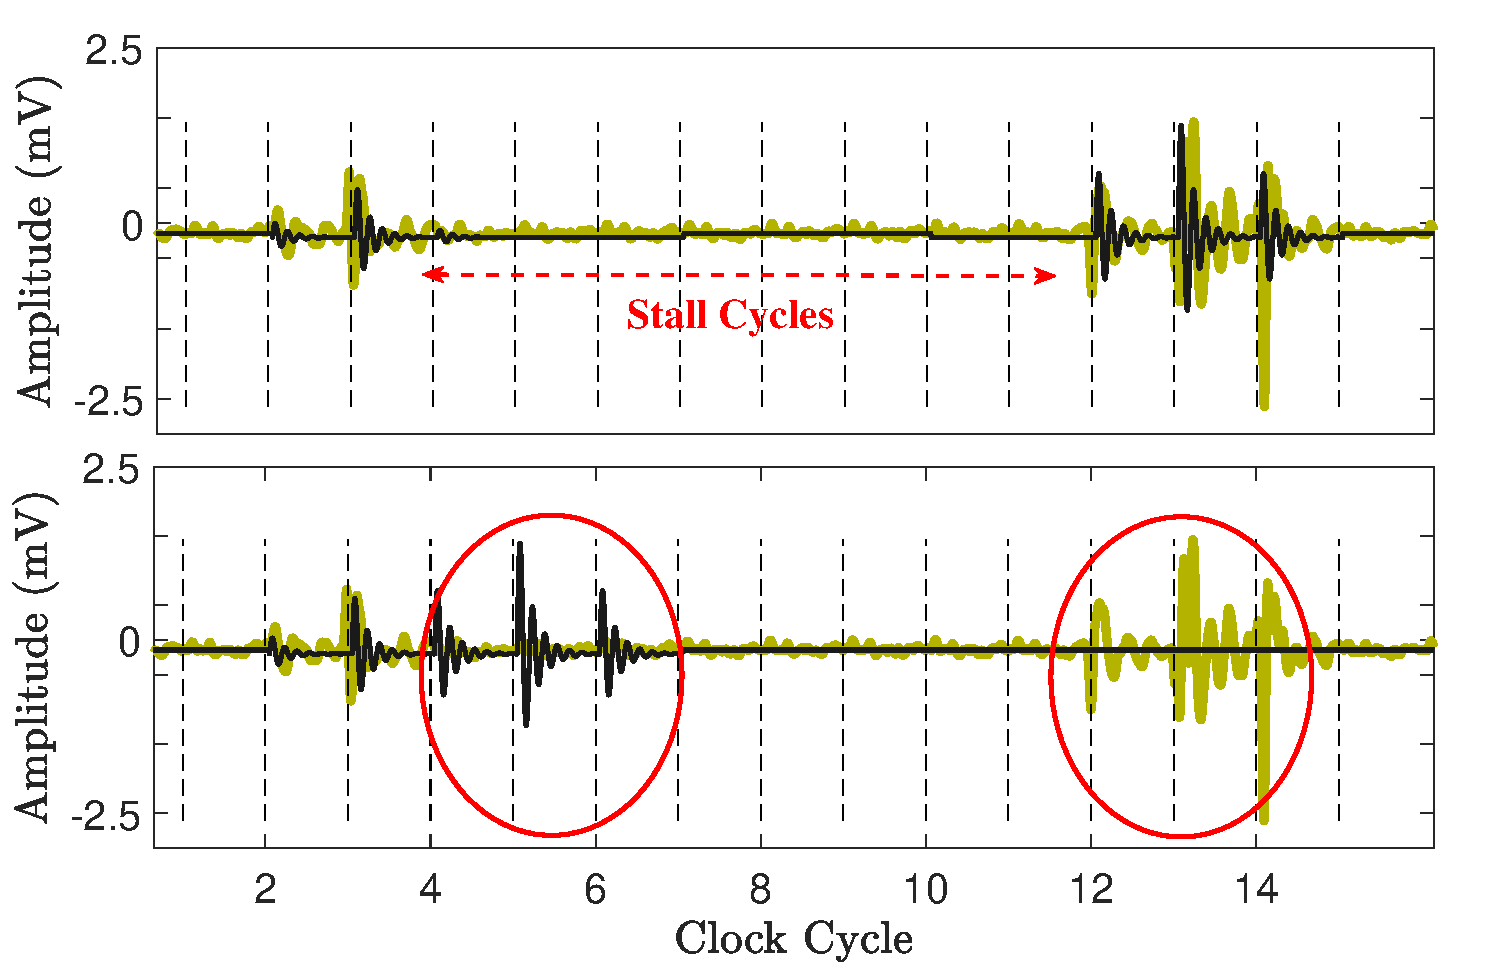
\includegraphics[width=0.4\columnwidth,clip]{figure/stall2.pdf}
	\caption{Effect of stalls on the signal. The actual signal shown in green, while simulated signals are shown in black when modeling pipeline stalls (top) and not modeling it (bottom).}
	\label{fig:stall}
\end{wrapfigure}

\noindent\textbf{Pipeline Stall}. Stalling is a common event in a processor which prevents successor instructions from advancing in the pipeline and preserves the instruction and operands in the stalled stages. Due to this preservation no bit-flips occur in the stalled stages. In addition, to save power, a control signal is typically used to disable (e.g., through power-gating) hardware components in the stalled stages. As a result, stalling typically has a dramatic impact on the switching activities of the stalled stages and, consequently, results in a significant reduction in the amplitude of the generated side-channel signals. Figure~\ref{fig:stall} shows the effect of stalling on the signal where a {\tt MUL} instruction has stalled the pipeline for eight cycles (we intentionally increased the stall cycles in {\tt MUL} for clarity). As can be seen from the figure, not properly simulating stalls (bottom) results in a significant deviation from the original signal (shown in light green).

Note that stalling does not have any impact on prior instructions thus they still generate side-channel signals as they advance through the pipeline. As a result, during stall the received side-channel signal is only generated by the instructions in the non-stalled stages (if any).

To properly model stalling, the simulator should be able to detect when stalls are happening (using the micro-architecture model), and ignores the signals generated by the stalled stages during the stall phase. In our model, this is done by setting the amplitudes of stalled stages to zero in Equ.~\ref{equ:miso}.\\
\begin{wrapfigure}{l}{0.4\textwidth}
	\centering
	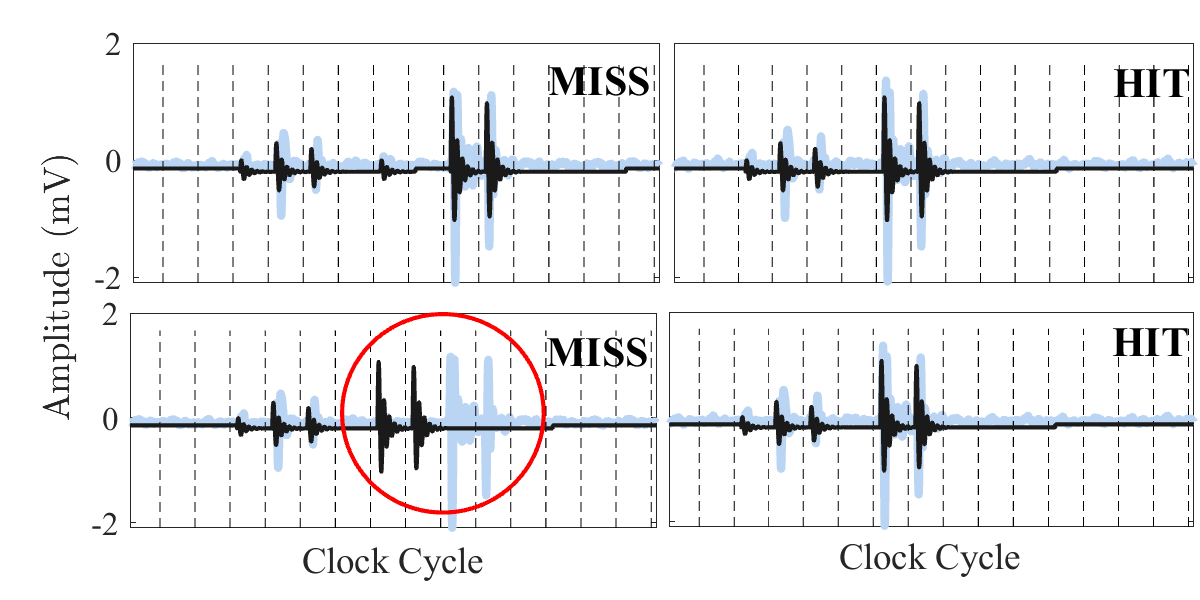
\includegraphics[width=0.4\columnwidth,clip]{figure/cache2.pdf}
	\caption{Effect of cache-miss (left) and cache-hit (right) on the signal. Miss causes two extra stall cycles. The actual signal (light blue) and simulated signals (black) with (top) and without (bottom) modeling cache misses are shown. }
	\label{fig:cache}
\end{wrapfigure}

\noindent\textbf{Cache miss}. Similar to pipeline stalls, due to a data-dependency, cache miss can also cause stalls. In our design, accessing the cache stalls the pipeline for one cycle. Further, cache miss and access to the memory causes extra two stall cycles. These two signals and their differences are shown in Figure~\ref{fig:cache}.

As can be seen in the figure, two extra stall cycles (total of three) can be seen in {\tt LD} instruction. Similar to stalls, the cache activity should be properly simulated using the micro-architecture model. Figure~\ref{fig:cache} illustrates how without properly modeling the cache misses the simulated signal will be deviated from the original signal (bottom left).    \\

\noindent\textbf{Misprediction}. In addition to stalls, we observed that branch misprediction also has noticeable impact on the side-channel signals. Depending on the pipeline design, the correct outcome of a branch instruction can be resolved after a few cycles (2 cycles in our design), and if a \textit{misprediction} is detected, the processor has to \textit{flush} the incorrectly fetched instructions, and begin executing the correct ones after that. In order to do that, processors typically substitute the incorrect instructions with {\tt NOP} instructions. It is expected that executing these \textit{bubble} instructions temporarily changes the side-channel signals since they change the switching activities of each stage. Figure~\ref{fig:mis} shows the received EM signals with and without a misprediction along with instructions present at each cycle in each pipeline stage.
\begin{wrapfigure}{l}{0.4\textwidth}
	\centering
	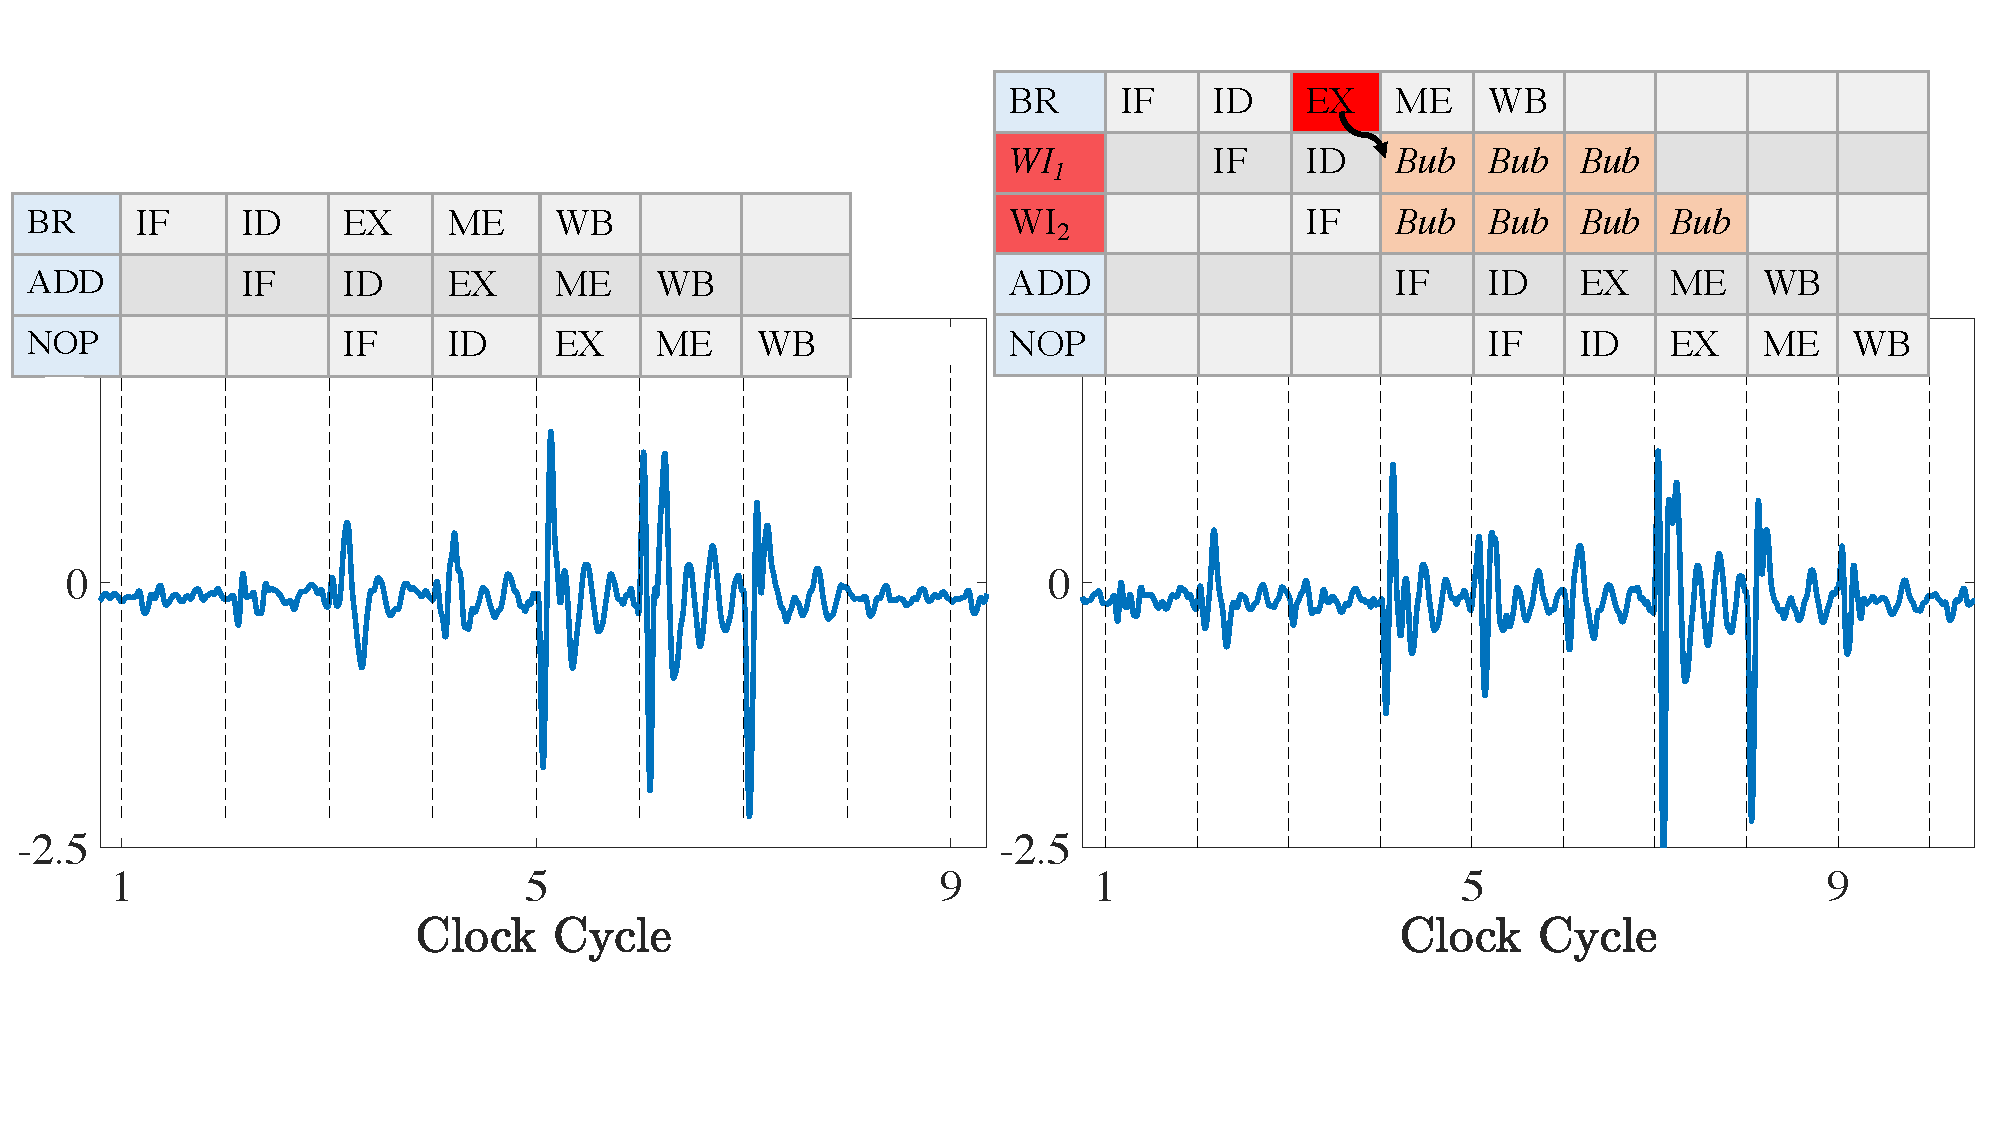
\includegraphics[width=0.4\columnwidth,clip]{figure/mise2.pdf}
	\caption{Effect of misprediction (right) on the signal. It causes two instructions being flushed from the pipeline and hence affect the signal in those cycles.}
	\label{fig:mis}
\end{wrapfigure}

Similar to pipeline-stall, using the micro-architecture model, mispredictions can be detected and simulated in our simulator. It is important to mention that we also studied the impact of using  different branch-predictors on the side-channel signals (e.g., always not-taken, 2-level, g-share, etc.) and we did not observe any statistically significant difference between these predictors mainly because they have relatively small switching activities (especially for low-end processors).

It is also important to mention that \textit{we tested the effect of other micro-architectural events} such as data-forwarding on the signal and did not observe any significant difference in the presence and/or absence of them. Also note that, as we mentioned before, in this paper, we limited the modeling to bare-metal, and left system-level activities modeling such as interrupts, exceptions, context-switch, etc., and advanced power-saving methods (e.g., DVFS, power gating, etc.) to future work.

\subsection{Evaluating Model Accuracy}
\begin{wraptable}{l}{0.6\textwidth}
\centering
\caption{RISC-V (R32IM) instruction-set and their cluster used in this paper.}
	\begin{tabular}{|c|c|l|c|}
		\hline
		\small Cluster& \small Type & \small Inst. & \small No. Inst. \\
		\hline
		1& \small ALU & {\tt ADD,XOR,JAL, ...}  & 13 \\
		\hline
		2& \small Shift & {\tt SLLI,SRT, SRA, ...}  & 10 \\
		\hline
		3& \small MUL/DIV & {\tt MUL, DIV, REM, ...} & 8 \\
		\hline
		4& \small Load & {\tt LB, LW, LH, ...} & 5 \\
		\hline
		5& \small Store & {\tt SB, SH, SW}  & 3 \\
		\hline
		6& \small Cache &  {\tt LB, LW, LH, ...} & 5 \\
		\hline
		7& \small Branch & {\tt BEQ, BLT, BGE, ...} & 6 \\
		\hline
	\end{tabular}
	\label{t:inst}
\end{wraptable}

\label{subss:eval}
\noindent\textbf{Setup}. We implemented a RISC-V based processor on a Terrasic DE0-CV board with an Altera Cyclone-V FPGA~\cite{de0} with 50 MHz clock-rate.  To record side-channel signals, we used a Keysight digital oscilloscope (DSOS804A), with 1 GHz bandwidth and 10 GSa/s rate. We further studied the effect of changing the sampling-rate on the accuracy and found that similar accuracy can be achieved with much lower sampling-rate (about 200 MSa/s in our measurements). As a result, similar results can be achieved using a less expensive device (e.g., TBS1032B Tektronix Digital Oscilloscope~\cite{oscTek} costs around \$300) and/or a high sampling-rate device can be used for modeling devices with faster clock-rates.

To receive EM signals, we used a magnetic probe~\cite{Antenna}, placed 5~cm above the FPGA. Signal processing is done in Matlab2017-b and the simulator is implemented in standard C++ programming language. \\

\noindent\textbf{Model Building}. In order to fit a model, \textit{ALL} possible combinations of instructions should be measured (i.e., about three hundred million combinations in RISC-V ISA). Clearly such a requirement makes the model building extremely time-consuming in practice.  However, intuitively, we expect instructions with similar behaviors (e.g., ALU-type, memory-type, etc.) have similar side-channel signals since they share identical hardware activities. Using this intuition, we used the \textit{hierarchical agglomerative algorithm}~\cite{frakes1992information} with the \textit{cross-correlation} as the distance metric to cluster instructions with similar EM pattern into a same cluster. We found that RISC-V ISA can be \textit{clustered} into 7 categories (when the operands are similar) where a single instruction in each category can be a representative of all instructions in that category.

These categories are shown in Table~\ref{t:inst}. Using this table, we then used only a \textit{representative} instruction of the cluster for model building which, in turn, reduce the model building complexity significantly. In our setup, the number of measurements was reduced from 300 million to only 16 thousands.  Note that while the clustering algorithm did not use the micro-architecture model as a prior knowledge, the clusters confirmed that instructions with similar micro-architecture activities should be clustered in a same group. \\

\noindent\textbf{Metric}. To measure how well the simulated signals ``match'' with the real signals, we leverage \textit{normalized cross-correlation} as our metric. To compute that, we first normalize both signals, real and simulated, to have similar average. We then divide each signal to individual clock cycles, and then compare each cycle (between the simulated and the real signals) using cross-correlation as the distance metric. We then define \textit{accuracy} as the average of this cross-correlation across all cycles for all measurements (i.e., we were able to match the waveform in this degree across all possible instruction sequences). Note that we specifically used this approach to show how well the time-domain signal \textit{matches} with the original signal instead of relying on a specific \textit{leakage metric} such as Hamming weight. However, to show the usefulness and versatility of our tool, those results will be shown in the next section.
\begin{wrapfigure}{l}{0.4\textwidth}
	\centering
	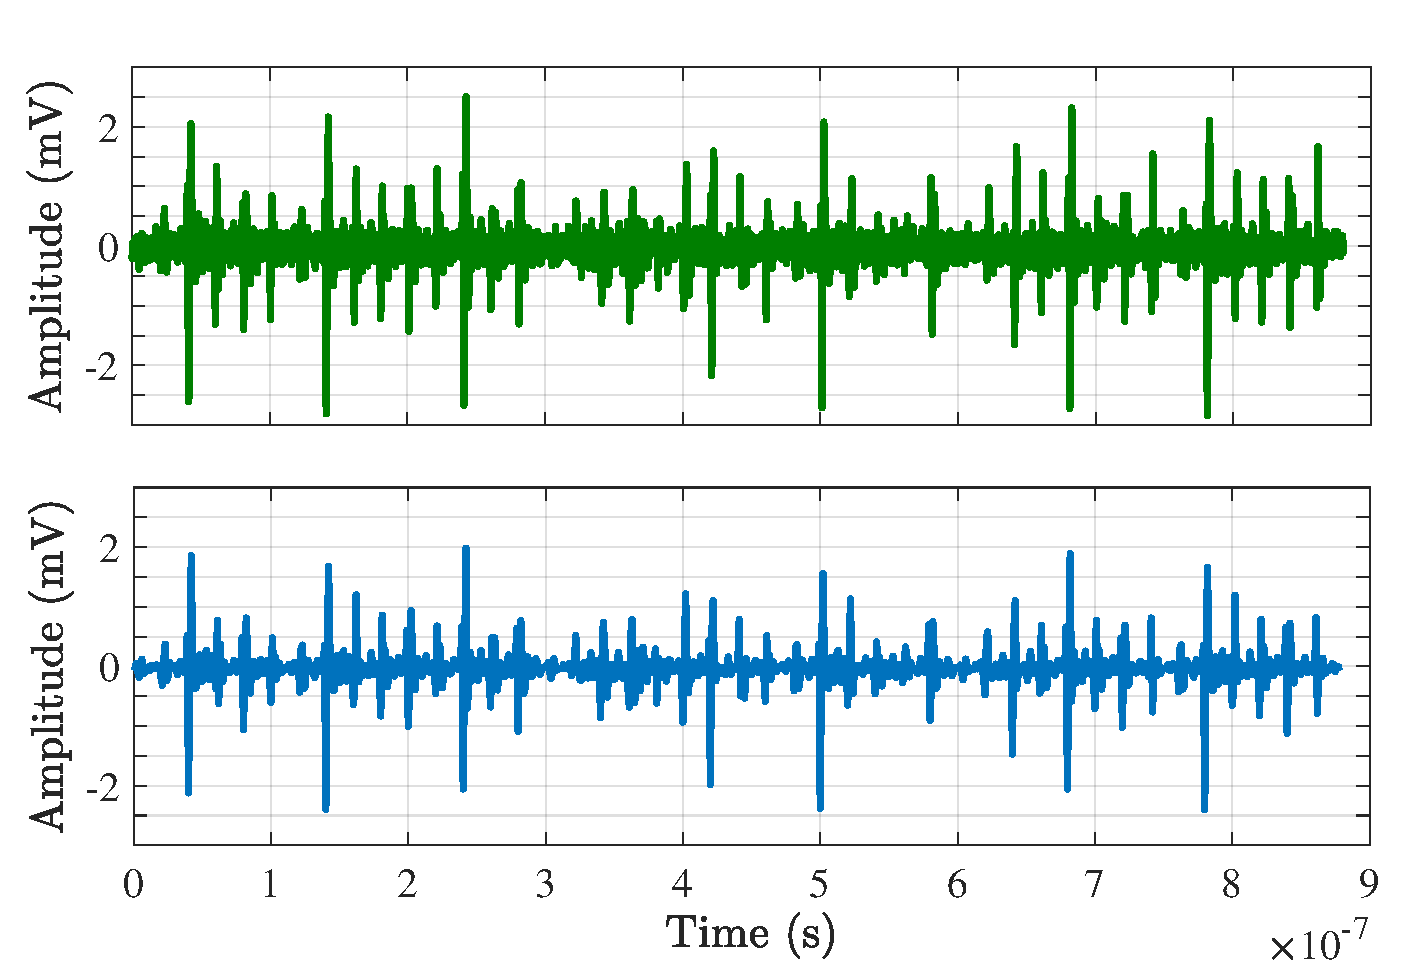
\includegraphics[width=0.4\columnwidth,clip]{figure/bench.pdf}
	\caption{A comparison between the signal generated by a real hardware (top) and the simulated signal (bottom) in EMSim.}
	\label{fig:bench}
\end{wrapfigure}

\noindent\textbf{Benchmark}. To prove that our approach provides accurate simulated signals for \textit{ALL} possible instruction combinations thus can be applicable to \textit{ANY} complex program that uses the mixture of the implemented ISA (R32IM), we created a microbenchmark using all possible combinations of the representative instructions shown in Table~\ref{t:inst}. Particularly, for a 5-stage pipeline and 7 distinct clusters, there are $7^5=16807$ possible combinations that can appear together (in the pipeline) in a cycle. We created a program to generate all these combinations with random operands. We then manually modified branch instructions and assigned the target address and branch condition to create loops with random instruction and iteration sizes.  To limit the execution time, we then randomly put these instructions into groups of 1024 combinations (i.e., 5120 instructions in each group which were executed one after another similar to a real program). To cover all the combinations, 17 of such groups were needed (no two groups were similar). We then executed these randomly-generated groups on the processor normally, and recorded the real and simulated signals. To further prove the validity and correctness of our simulator, we also randomly created another 17 groups, this time from all  instructions in the ISA and not just the representatives. \\

\noindent\textbf{Results}. Using these 34 groups/applications described above, we then compared the simulated signals with the actual ones using the our metric defined earlier. Each group/application takes about 9000 cycles to finish on average. The execution-time varied depending on the instructions used and microarchitectural events.

Figure~\ref{fig:bench} shows the simulated and actual EM-side-channel signals for one of the groups tested in our evaluation (for clarity, only the first 50 cycles are shown in the figure). As can be seen from the figure, the simulated signal matches the real signal with high accuracy. We found that, on average, \textbf{\textit{EMSim has about 94.1\% accuracy in simulating side-channel signals across all possible instruction combinations}}.

\color{red}
\subsection{Enabling Side-Channel Aware Software Development}
Most software developers lack both the know-how and the equipment to evaluate
their software's potential vulnerability to analog side channels.  As such,
blackbox software which enables developers to analyze their software for analog
side channels is valuable. To enable this type of software analysis, we have
developed a framework which performs symbolic execution of a program on a
detailed (gate-level) model of a microprocessor~\cite{cherupalli2017}.
This framework was originally developed in order to automate design of
`bespoke microprocessors' --- microprocessors designed to execute a single
application binary. The flowchart for this use case is in Fig.~\ref{fig:bespoke}.
The symbolic execution of the program on the hardware occurs in the
`Gate Activity Analysis' stage.

\begin{wrapfigure}{l}{0.4\linewidth}
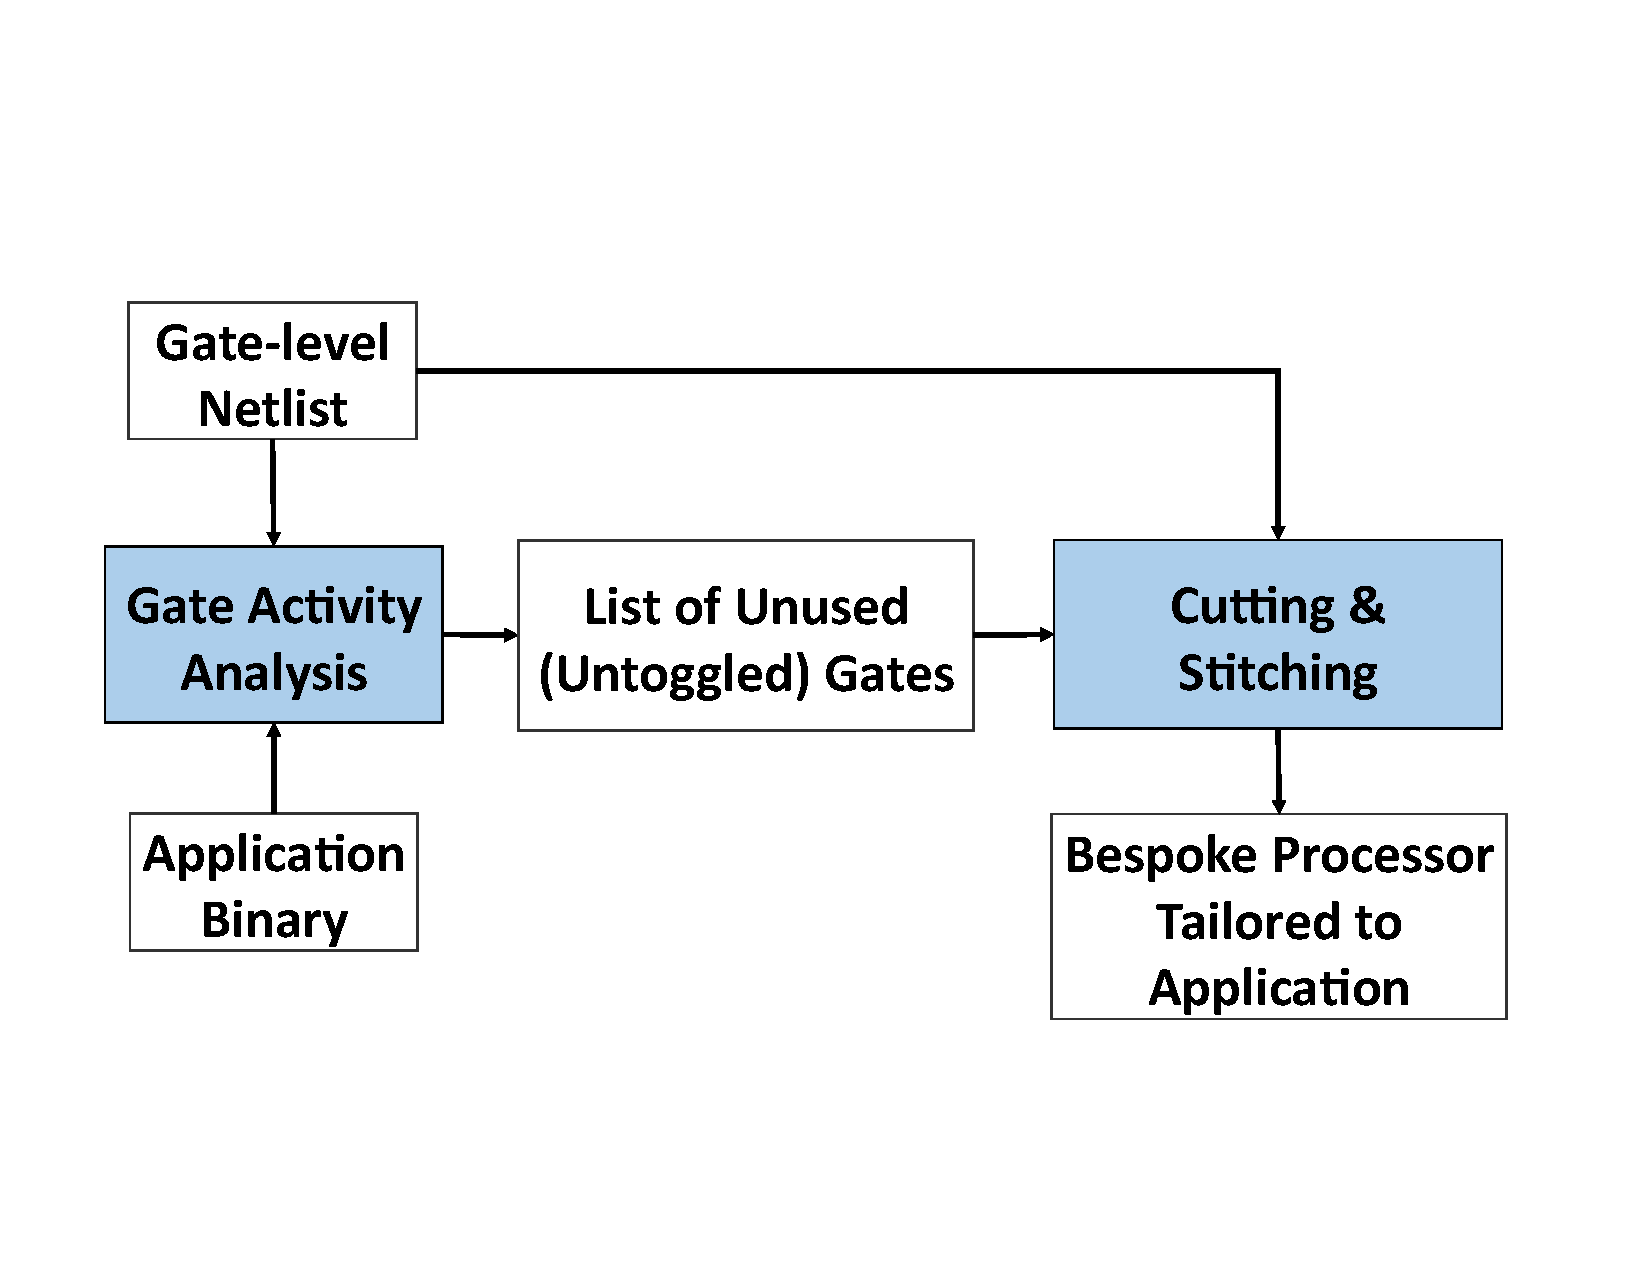
\includegraphics[width=\linewidth]{./figure/Bespoke_Flow_Fig.pdf}
\caption{\small
    Hardware-software co-analysis used to generate bespoke microprocessors.}
\label{fig:bespoke}
\end{wrapfigure}

Program execution is affected by program inputs (e.g., sensor inputs) and
different inputs can result in not just variation in data-dependent activities
(i.e., switching activities on data and address busses), but also variation in
instruction-dependent activities due to input-dependent branch instructions.
This symbolic execution framework allows us to identify whether any possible
execution of a program leads to an EM side-channel which leaks sensitive
information. Security is a critical consideration for processors in the IoT
space.
However, many IoT devices cannot afford to run advanced security
protocols due to energy constraints. Our symbolic execution framework will
allow us to identify when a program is susceptible, and, importantly, when it
is not susceptible to an EM side-channel attack, allowing us to add or remove
the often expensive software based techniques to mitigate side-channel attacks
as needed.

Our framework has shown applicability for security
applications~\cite{cherupalli20172}. We have demonstrated its use in
taint-tracking for information flow security to locate information policy
violations, even violations which result from covert timing side-channels.

\color{black}

\color{red}
\subsection{Enabling Side-Channel Aware Hardware Development}
While analysis of \textit{software} can be done using symbolic execution of the
software alongside a model of the hardware, symbolic execution is not a useful
tool for hardware designers attempting to determine if there exists
\textit{any} program which can leak information via a side-channel (i.e.,
symbolic execution cannot be used to determine if side-channel mitigation
techniques are adequate for \textit{all} possible programs).  This is because
symbolic execution considers all possible executions of a single program, not
all possible executions of all possible programs. In order to address this
shortcoming, we have developed a hardware model checking framework which
analyzes net switching behavior for arbitrary programs~\cite{bleier21}. This
was originally designed to generate microprocessors optimized to certain ISA
subsets.  Fig.~\ref{fig:pdat} shows an overview of this process, which we
call Property Driven Automatic Transformation (PDAT).
The inputs to PDAT are the microprocessor's
netlist, and two collections of properties.  The first, the `Property Library',
is a collection of properties for each type of gate in the netlist.  These
properties are used to capture gate switching activities.
The final input, the environmental restrictions, are properties describing
the possible inputs to the microprocessor (including all possible programs
and program data).  The environmental restrictions are used to ensure that
the model checkers only consider valid or legal programs and inputs, rather
than arbitrary programs and inputs.

\begin{wrapfigure}{l}{0.6\linewidth}
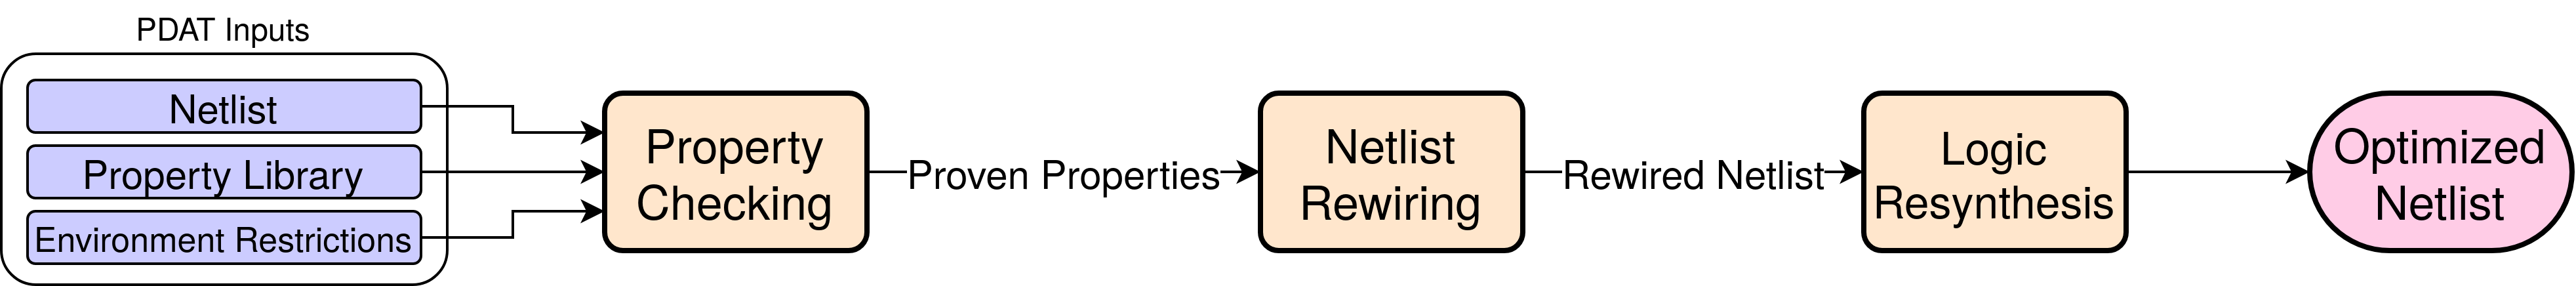
\includegraphics[width=\linewidth]{./figure/PDAT.png}
\caption{\small
    Model checking is used to identify gate switching behavior, and modify
    hardware appropriately.
}
\label{fig:pdat}
\end{wrapfigure}

Using model checking, in conjunction with microarchitectural hardware models,
designers can determine whether their design is resilient to EM side channel
leakage.  Since model checking provides witnesses to its proofs, it can
identify sequences of instruction/instruction classes and microarchitectural
events which lead to leakage of information via EM side-channel. PDAT, like the
symbolic execution framework which was originally intended to generate bespoke
microprocessors, may be repurposed to identify EM side-channel signatures.

\color{black}


% \color{red}
Most software developers lack both the know-how and the equipment to evaluate
their software's potential vulnerability to analog side channels.  As such,
blackbox software which enables developers to analyze their software for analog
side channels is valuable. Analysis of a \textit{program} is difficult
vis-\`a-vis analysis of an \textit{single execution} of the program, because
analyzing the program means analyzing all possible executions of the program.
In fact, program inputs can also effect microarchitectural events (e.g.,
stall due to branch predictor miss on data-dependent branch, cache hit/miss
based on input-dependend data accesses, etc).  It is possible that
one program execution does not result in leakage of sensitive information
via analog side channel, while a different execution of the same program
does result in leakage of sensitive information via analog side channel.
As such, it is important for developers to be able to
analyze \textit{all} possible executions of their programs.

The PIs previous work using symbolic execution of programs to analyze net
switching behavior~\cite{cherupalli2017} and perform taint
tracking~\cite{cherupalli20172} is highly relevant, as it enables capturing
switching activities for all possible executions of a given program.  The prior
work can be modified to meet the abstraction level of the microarchitectural EM
side channel model (Sec.~\ref{sec:preliminary_results}).
Developers will be able to use this symbolic execution framework to perform
microarchitecturally aware analysis of their software's susceptibility to
analog side channel information leakage without any additional expertise or
equipment (in fact, they will not even need the targetted microprocessor).



\section{Proposed Research}



\textbf{Machine learning methods for analog side channel modeling}. In this task we propose to develop machine learning techniques that will allow for analog side channel modeling that is not dependant on collecting measurements on particular processor and are scalable across different processor and memory speeds. Furthermore, we propose to create neural network structure that does not require to observe all possible combinations of instructions in order to model larger sequences of instructions. Finally, we propose to develop methods for ``calibration'' of simulation parameters against measured signals from real systems.

\color{red}
Our symbolic execution framework, used to enable side-chanel aware software
development, currently uses detailed gate-level models of the microprocessor
hardware.  This approach results in high fidelity reproduction of the
microprocessor's EM side-channel, but comes at a high computational cost,
limiting its utility to a software developer.
For example, an FFT implementation for a 16-bit MSP430 DSP takes over 10,000
seconds to run on the gate-level framework.  This means that a developer would
need to wait nearly three hours between modifying the program, and getting
results for its impact on EM side-channel information leakage.  We will raise
the abstraction level of our symbolic execution framework from the gate-level
to the MISO model abstraction detailed in Sec.~\ref{sec:preliminary_results}.
There are several pecularities which make this an interesting task.  First,
data-dependent activities will often be evaluated for symbolic data.  As such,
for a given time period, the EM signal is best modeled as a distribution.
Second, microarchitectural events (i.e., stalls, cache misses, and branch
mispredictions) will also be dependent on symbolic data (e.g., a symbolic
address resulting in either a cache hit or a cache miss).  Thus, great care
must be taken to ensure the path explosion problem is not exascerbated by the
modeling of microarchitectural events.  These pecularities mean that performing
symboilc execution at the MISO model level is not straightforward,
hence enabling side-channel aware software development requires further
research effort.
Additionally, identifying relevant information flow policies and determining
the EM characteristics associated with violations of the policies requires
further effort.
\color{black}



\color{red}
We will create a version of PDAT purpose built for identifying potential EM
side-channel leakage using the high-level MIMO model, rather than a detailed
netlist model. Unlike symbolic execution, model checking does not suffer from
the path-explosion problem (model checking's computational complexity is based
on the size of the model's state space), thus handling microarchitectural
events poses no significant difficulties. Since the high-level model has
significantly smaller state-space than a microprocessor's netlist, this will
lead to significant decrease in model checking runtime.
It will also enable computer architects to
rapidly explore the architectural design space for EM side-channel behavior.
For example, an architect can determine the impact of branch delay
slots~\cite{lalja88} on side-channel behavior by disabling the branch
misprediction event within PDAT, or determine the impact of software based
multiplication by restricting the execution environment to non-multiply
instructions.

PDAT's environment restrictions allows us to also use PDAT for
software-hardware co-analysis.  We can restrict the environment to a single
program, and use model checking to explore all possible executions of the
program for a given hardware model.  This enables hardware-software codesign
flows to be EM side-channel aware.

A model checking approach can also be used purely by software developers, as an
alternative to the symbolic execution approach, by restricting the execution
environment to a single program.  As the performance of model checking and
symbolic execution are both dependent on the particular MISO model as well as
the particular program, it is likely that in some cases, symbolic execution
will perform better than model checking, and vice versa.  This makes both
approaches to side-channel aware software development valuable.
\color{black}



\color{red}
We have experience with not just digital design, but chip design,
tape-out, and testing, and run an undergraudate course in which student designs
are manufactured by TSMC and then tested on campus.  We also participate
in Intel's Chip Design Challenge, manufacturing RISC-V microprocessors in Intel
16 nm technology. This provides the PIs a sizeable collection of
microprocessors with various microarchitectures which can be profiled at
multiple levels of abstraction - high-level microarchitecture, RTL, gate-level,
GDS/geometry level, and physical chips. This allows the PIs to evaluate the
predictive accuracy of the model described in
Section~\ref{sec:preliminary_results} when modified for other ISAs and
microarchitectures, and calibrate the model builder based on real-world designs
and implementations.
\color{black}



\section{Integrated Research, Education, and Outreach Plan- EDIT}
The research, education, and outreach milestones for each year are outlined in the following table.
\begin{small}
\begin{tabular}{||c|p{0.42\linewidth}|p{0.42\linewidth}||}
\hline
\hline
\textbf{Year} & \textbf{Research} & \textbf{Education and Outreach}\\
\hline
\textit{1} &
  &
Develop initial modules for graduate courses, visits to local schools, undergraduate teams work on lab measurement setups\\
\hline
\textit{2} &
&
Develop course modules for graduate and undergraduate courses; visit school for hands-on demonstrations, undergraduate teams experiment with refinements to measurement, training, and matching methodology \\
\hline
\textit{3}  & 
 &
Refine course modules; develop K-12 and public demonstrators for sensory experiences of HT detection (e.g., use software defined radio setups to demonstrate HT detection); fully integrate undergraduates in research\\
\hline
\hline
\end{tabular}
\end{small}

The PIs plan to conduct the proposed research in a highly integrated manner.
Three PhD students will work on this project, and we will seek out students
whose primary expertise is in one of the areas relevant to this project,
but who are willing to learn and contribute to the other areas. We also
anticipate that most (or all) of the students will be co-advised. Finally,
we will hold weekly meetings to both keep the project well-coordinated and
to foster exchange of ideas across the disciplines involved in this project.

Our interdisciplinary approach requires technical and research
expertise from several Computer Science (CS) and Electrical Engineering (EE) disciplines, and each PI brings skills essential for the success of this work.

\color{red}
The MISO abstraction symbolic execution framework as well as MISO-based PDAT
framework will be open-sourced. This will allow other researchers to perform
side channel analysis for their designs.  Runtime power estimates from high
level simulation and circuit level simulation as well as measurements from
prototyped chips will be made available as well. This data can be helpful for
wide variety of research.

This work will train several graduate and undergraduate students in a unique
and up-and-coming interdisciplinary area at the intersection of architecture,
tool development, and signal processing – this training will help add to a
unique workforce.  Undergraduate researchers working with PI Kumar have
recently published in premiere computer architecture conferences, including
ISCA, HPCA, and DAC. ISCA paper was covered widely by media. HPCA paper was
nominated for a Best Paper Award; DAC paper received significant media
coverage. Several undergraduate researchers have gone on to join graduate
studies at UIUC and elsewhere. The nature of the project will help us engage a
large number of undergraduate students in research.

Dr. Kumar has assisted in the organization of events such as HackIllinois and
Engineering Open House (EOH) that see enthusiastic participation from the local
community. He will have a booth on “processors that leak information” in the
next three EOHs to get high school students excited about intersection of
computer architecture and security.

Dr. Kumar was recently awarded the Ronald W Pratt Faculty Outstanding Teaching
Award and Stanley H Pierce Faculty Award at UIUC for, among other things,
innovative teaching of project-based courses in computer architecture and
system design. He also recently co-created a course on chip design and tapeout
where student groups perform tapeout of chips which then get manufactured by a
commercial foundry. Groups then do testing and bringup. The tapeout work
supporting the project will be done in context of this this course. Dr. Kumar
will blend in a discussion of side channel information leaking processors and
accelerators in his graduate computer architecture class. He will also list
side channel analysis and mitation related projects as project options in the
class, while making available the tools developed in this research.
\color{black}



\subsection{Proposed Outreach and Education Activities}

In addition to research proposed here, this proposed work will help foster interaction among researchers from a
very diverse set of research areas and will involve training students
with a considerable multidisciplinary expertise. To further increase
the impact of this work, we are also planning to perform the following
outreach and education activities.

\begin{itemize}\denseitems

\item We will introduce relevant cross-disciplinary material into
  several courses at the graduate and undergraduate level. For
  example, we will add to VLSI and computer
  architecture courses an introduction to physical side-channel (EM)
  signals. Similarly, in electromagnetics, telecommunications, and
  signal processing classes, we will add a discussion of how computer
  hardware and software interact to create side-channel signals. This
  will help students understand the broader perspectives relevant to
  each class, and also help them appreciate the increasingly
  multi-disciplinary nature of science and technology.

\item We will continue to include undergraduate students in our
  research. The PIs Zajic and Prvulovic have long history of advising undergraduate students (26 undergrads) through
  Opportunity Research Scholar (ORS) program at Georgia Tech and individual motorship and plan to continue that activity.

\item Another outreach activity will be the development of displays
  and tools for educating the general public, especially high-school
  students and teachers, on issues related to both HTs and side-channel signals. This initiative will be
  pursued through Georgia Tech’s established outreach programs for
  high schools in the greater metro Atlanta area~\cite{Conrad2022}.
  The PIs Zajic and Prvulovic have done this in the past with hands-on demonstration for the Family Science Night at the Mimosa
  Elementary School in Roswell, GA and hands-on STEM activities at Pace Academy in Atlanta, GA.
\end{itemize}


\section{Results from Prior NSF Support}
\label{sec:prior}
\noindent
{\bf Dr. Prvulovic and Dr. Zajic} have served as PIs and Co-PIs on the following NSF-funded projects in the last five years CCF-1563991 SHF (from 2016-2022 $\$850K$) and CNS 1740962 (from 2017-2019, $\$199,866$).

Grant CCF-1563991 SHF \textit{Spectral Profiling: Understanding Software Performance without Code Instrumentation}
($\$850K$, October 2013- September 2016).
\textit{Intellectual Merit:}Our seminal work on EM emission based program profiling provided the basis for
future work in the more general area of program analysis techniques that leverage the physical side
effects of computation \cite{Zop, Zop2, Nader2016, Elvan2021}.
\textit{Broader Impact:}This work has opened up new possibilities in a number of additional areas,
including program testing and debugging and software security. Inherently interdisciplinary, research has improved the state of the art in many areas including electromagnetic, signal processing, computer architecture, and software engineering.

Grant CNS 1740962\textit{EAGER: Exploration of THz Backscattering
as a Side-channel in Computer Systems}
($\$107K$, September 2010--August 2012).
\textit{Intellectual Merit:}Our seminal work on backscattered signals and how they can be used for HT detection has opened up new possibilities
for non-destructive testing of electronics and for more precise detection of dormant HTs \cite{Pavel2020,nguyen19,Erik2022}.
\textit{Broader Impact:}THz back-scattering side-channel is an entirely new side channel that significantly differs
from existing ones for both defensive and offensive uses. We have built several testbeds and demos and demonstrated it to various communities
to educate public about this new technology. We have received several best paper and patent awards.

{\bf Dr. Zajic} is currently also the PI on grant ECCS-1651273 NSF CAREER(from 2017-2023 $\$500K$) \textit{Modeling and Measurements for THz Wireless Chip-to-Chip Communications Propagation} \textit{Intellectual Merit:}To enable future THz wireless communication between chips in a system and between blades and racks in large-scale data center systems, this project is investigating  propagation mechanisms \cite{Cheng2020}, \cite{Kim2016}, \cite{Fu2019} and develops channel models \cite{Kim2016a}, \cite{Fu2020} to enable communication between chips on a motherboard inside a computer system, between the motherboard and an add-on card (e.g., a graphics card), between boards/blades in a rack-mounted system typical for base stations, and between racks in a data center environment (with raised floors, rows of racks, cooling ducts, etc.). \textit{Broader Impact:} In addition to the broader impact within the research community and training graduate students funded by this grant, the PI is leading mm-wave indoor channel modeling and measurements efforts in the 5G Millimeter Wave Channel Model Alliance, led by National institute of Standards and Technology, which aims to produce more accurate, consistent and predictive channel models for frequencies above 6 GHz and lead the standardization process \cite{Book}.

\color{red}
Dr. Kumar has served as PI on the following NSF-funded project in
the last five years: CCF-2006763 SHF (from 2020-2023 \$500K).

CCF-2006763 SHF Printed Computer Systems (\$500K, October 2020- September
2023). Intellectual Merit: The project has already resulted in first sub-cent
microprocessor~cite{bleier22}, first plastic encryption
engines~\cite{bleier23}, first work on printed
microprocessors~\cite{bleier2020printed}, and first work on printed
classifiers~\cite{mubarik20}. Broader Impact: This project has opened up new
possibilities for ultra-low cost and conformal active electronics, enabling
applications such as wearable patches~\cite{8502791},
garments~\cite{garments},
packaging~\cite{gethin2013printed} for fast
moving consumer goods (FMCG), low-end healthcare products such as smart
bandages~\cite{DERAKHSHANDEH20181259},
and disposable sensors for food~\cite{7994325},
pharmaceuticals~\cite{BERGAMINI200554},
agriculture and forestry~\cite{chemosensors8040125},
and environment~\cite{MARRAZZA1999297} --- that have not seen much
penetration of computing.
\color{black}


\bibliographystyle{abbrv}
\bibliography{refs}
\end{document}

